\documentclass[11pt]{article}
\usepackage{fullpage,amsthm,amsfonts,amssymb,epsfig,amsmath}
\usepackage{multicol}
\usepackage{soul}

\begin{document}

\begin{center}
{\bf\large HW4 - S16}\\
Handed out 4-20 \hfill Chris Troiano \hfill 4-26, beg. of class \\
\end{center}

\begin{enumerate}
\item$\;$
(a) Run Dijkstra's algorithm on the following graph (showing all
intermediate steps).\\
(b) Show the shortest path tree corresponding to running Dijkstra on
this graph.\\

{\bf Solution:}\\
\begin{enumerate}
\item Table:
\begin{table*}[h]
\renewcommand{\arraystretch}{1.3}
\caption{Dijkstra's Shortest Path}
\label{tab:Dijkstra's}
\centering
\begin{tabular}{c|c|c|c|c|c|c|c|r|l}
iteration & A & B & C & D & E & F & G & H
\\ \hline \hline
0 & 0 & $\infty$ & $\infty$ & $\infty$ & $\infty$ & $\infty$ & $\infty$ & $\infty$ \\
1 & 0 & 1 & $\infty$ & $\infty$ & 2 & 10 & $\infty$ & $\infty$ \\
2 & 0 & 1 & 2 & $\infty$ & 2 & 6 & 4 & $\infty$ \\
3 & 0 & 1 & 2 & 7 & 2 & 4 & 3 & $\infty$ \\
4 & 0 & 1 & 2 & 7 & 2 & 4 & 3 & 10 \\

\end{tabular}
\end{table*}

\item Graph:\\
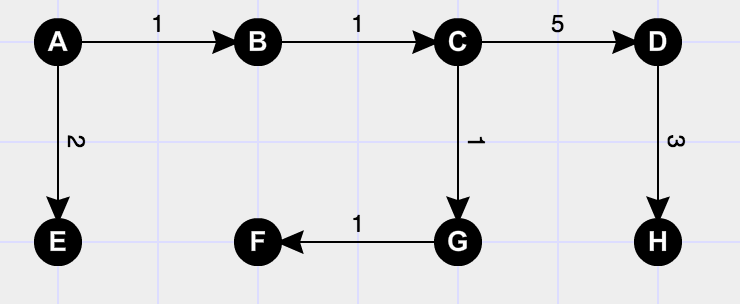
\includegraphics[width=2in]{2ndgraph.png}
\end{enumerate}

\item$\;$
 Run Kruskal's algorithm on the following graph (showing all
intermediate steps).\\

{\bf Solution:}\\
Edges ordered by weight:\\
\begin{multicols}{3}

%$A - E: 1$ \hspace{1.5cm} \st{$B - E: 5$}\\
%$A - B: 2$ \hspace{1.5cm} \st{$C - F: 5$}\\
%$B - F: 2$ \hspace{1.5cm} \st{$D - G: 5$}\\
%$C - D: 3$ \hspace{1.5cm} $G - H: 6$\\
%$F - G: 3$ \hspace{1.5cm} \st{$B - C: 7$}\\
%$C - G: 4$ \hspace{1.5cm} \st{$D - H: 7$}\\
%\st{$E - F: 4$}

$A - E: 1$\\
$A - B: 2$\\
$B - F: 2$\\
$C - D: 3$\\
$F - G: 3$\\
$C - G: 4$\\
\st{$E - F: 4$}\\
\st{$B - E: 5$}\\
\st{$C - F: 5$}\\
\st{$D - G: 5$}\\
$G - H: 6$\\
\st{$B - C: 7$}\\
\st{$D - H: 7$}\\
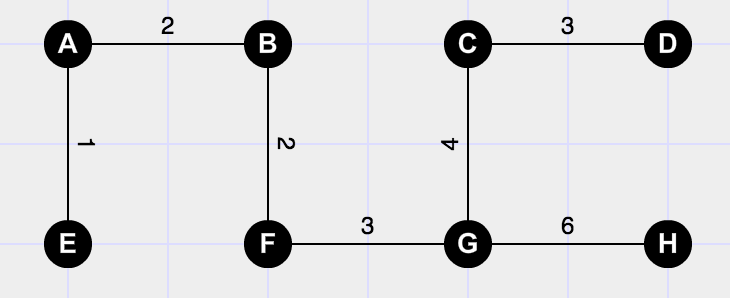
\includegraphics[width=2in]{1stgraph.png}

\end{multicols}

\item
\begin{enumerate}
\item
Consider the edge $(B,E)$ in the graph of Problem 2.
Either show that there is a minimum cost spanning tree using
this edge by applying the cut property, or
prove that this edge is not used in any minimum cost
spanning tree using the cycle property.
\item
Ditto for edge $(C,G)$.
\end{enumerate}

{\bf Solution:}\\
\begin{enumerate}
\item
Observe cycle ${A, B, E}$\\
\begin{center}
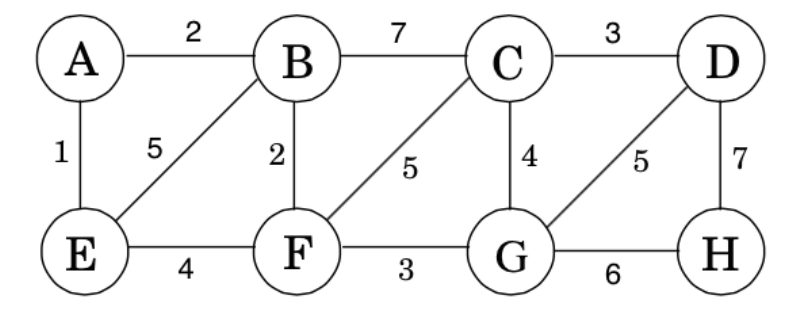
\includegraphics[width=2in]{copy.png}
\end{center}
\begin{multicols}{2}
$A - E: 1$\\
$A - B: 2$\\
$B - E: 5$\\
\vfill
\columnbreak
By the cycle property, $B - E$ is not in the MST.
\end{multicols}

\item
Let $S$ be the subset of nodes ${C, D, H}$. The cutset contains edges:\\
\begin{multicols}{2}


$B - C: 7$\\
$C - F: 5$\\
$C - G: 4$\\
$D - G: 5$\\
$G - H: 6$\\

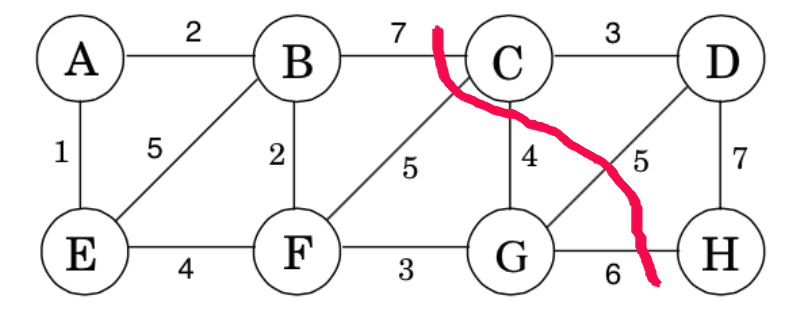
\includegraphics[width=2in]{cutset.png}
\end{multicols}
$C - G$ is the min cost edge with exactly one node ($C$), in $S$. Therefore the MST contains the $C - G$ edge.

\end{enumerate}
\item
Prove or disprove the following statements about an
arbitrary undirected graph $G=(V,E)$:
\begin{enumerate}
%\item The shortest-path tree computed by Dijkstra’s algorithm is necessarily
%an MST.
\item If e is part of some MST of G, then it must be a lightest edge
  in some cutset of G.
\item If graph G has more than $|V | - 1$ edges, and there is a unique
  heaviest edge, then this edge cannot be part of a minimum spanning
  tree. 
\item The shortest path between two nodes is necessarily part of some MST.
\end{enumerate}
{\bf Solution:}\\
\begin{enumerate}
\item
Let $S$ be a subset of nodes in $G$ where edge $e$ has exactly one endpoint in $S$. Let $T$ be a MST of $G$ that does not contain $e$. When we add $e$ to $T$, it creates a cycle $C$. Edge $e$ is in the cycle $C$ \& the cutset $X$. There exists another edge $l$, that is in both $C$ \& $X$.\\
$T^{\prime} = T \cup \{e\} - \{l\}$ is also a spanning tree.\\
$e < l, cost(T^{\prime}) < cost(T)$, therefore, e is the lightest edge in cutset $X$.
\newpage
\item
This is false because the longest edge may be the only edge connecting some node to the MST and thus, must be included.\\

\begin{center}
%\begin{multicols}{2}
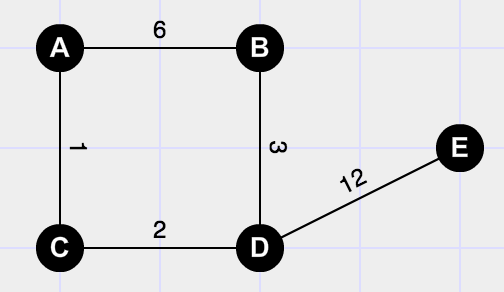
\includegraphics[width=2in]{before.png}
$\Rightarrow$
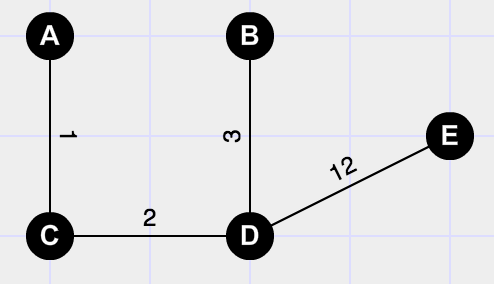
\includegraphics[width=2in]{after.png}
%\end{multicols}
\end{center}

\item
This is false, consider the undirected graph below. The shortest path between $A$ \& $C$ is $1.5$, but if Kruskal's algorithm is used to find the MST, it will be composed with the two lighter edges.

\begin{center}
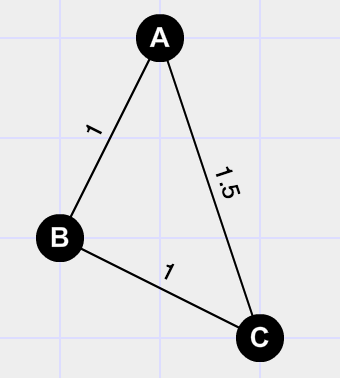
\includegraphics[width=1.5in, height=1.5in]{before1.png}
$\Rightarrow$
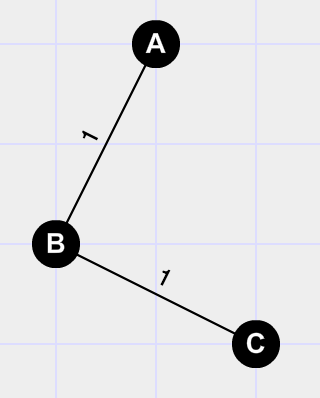
\includegraphics[width=1.5in, height=1.5in]{after1.png}
\end{center}
\end{enumerate}


\item
Consider an undirected graph $G=(V,E)$ with non-negative
edge weights $w_e\ge 0$. Suppose that you have computed a
minimum spanning tree of $G$, and that you have also
computed shortest paths to all nodes from a particular
$s\in V$.

Now suppose each edge weight is replaced by $w_e'=f(w_e)$,
where $f$ is a strictly increasing function.
\begin{enumerate}
\item
Does the minimum spanning tree change? Give an example
where it changes or prove that it cannot change.
\item
Do the shortest paths change? Give an example where they
change or prove they cannot change.
\end{enumerate}
{\bf Solution:}\\
\begin{enumerate}
\item
If each edge weight is replaced by $w_e'=f(w_e)$, the MST will not change. This is best illustrated with Kruskal's algorithm. If we order the all the edges, $w_e$, they will stay in the same order when we apply the strictly increasing function $w_e'=f(w_e)$, we know this because the function is strictly increasing and not sinusoidal or decreasing. Therefore, the algorithm will produce the same MST.

\item
The shortest paths can change. Consider the graphs below:
%\begin{multicols}{3}

\begin{center}
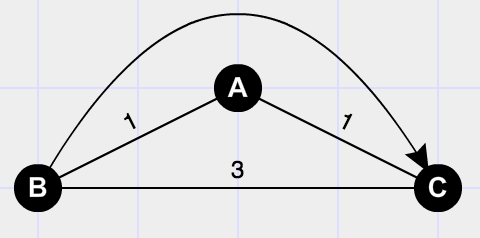
\includegraphics[width=2in]{before2.png}
$f(w_e)=w_e+2$
$\Rightarrow$
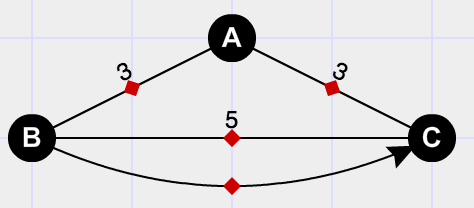
\includegraphics[width=2in]{after2.png}

\end{center}
Initially the shortest path from $B - C$ is $B - A$ then $A - C$. After applying the strictly increasing function to each node, the shortest path is now $B - C$.
%\end{multicols}
\end{enumerate}


\item
{\bf Extra Credit}. 
Let $G=(V,E)$ be a directed graph. A path $(v_1,v_2,\dots,v_n)$ in $G$
is called a {\bf simple path} if it does not have cycles, meaning that
no node repeats twice in the path. Note, that for the shortest path
problem with non-negative weights, any shortest path will always be a
simple path. This may not be the case when we allow negative
weights. For the purpose of this problem however, we will consider the
problem of finding the {\bf shortest simple paths} from a given source.

It is known that Dijkstra's algorithm may not
return the correct result to this problem if a graph contains edges
with negative weights. What if we only allow negative weights on the
edges leaving 
the source node (and all other edges are guaranteed to have
non-negative weights)? Will Dijkstra's algorithm be always correct in
this case (for finding shortest simple paths)? If yes, prove it, if no, provide a counter-example.
\end{enumerate}
{\bf Solution:}\\
Dijkstra's algorithm will not always be correct. Consider a graph where there is a relatively large negative edge weight involved in a cycle. The algorithm will find that every time around the cycle, the cost of the path gets smaller.\\
\begin{center}
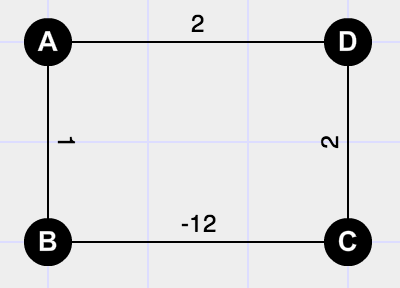
\includegraphics[width=2in]{cycle.png}
\end{center}


\end{document}
